\subsection{Arquitectura del sistema}
\label{subsection:impl_propia}

	El enfoque del presente trabajo se centra en los problemas de reconocmiento de caracteres y el reconocimiento de palabras. En las próximas subsecciones, se procederá a explicar cuestiones de implementación que se tuvieron en cuenta al momento de resolver ambos problemas.

	\subsubsection{Reconocimiento de caracteres}
		\label{subsubsection:recon-caracteres}
	
	
	\paragraph{Pipeline de procesamiento} ~\\

			La implementación que se realizó en este trabajo, está basada en un pipeline similar al que realizaron Wang et al. que comprende dos instancias: la instancia de entrenamiento y la instancia de evaluación. La primera esta constituida por la generación de datos sintéticos que constituyen el conjunto de entrenamiento, la extracción de las características, la binarización y el entrenamiento del clasificador. La segunda instancia consiste en la evaluación del clasificador que abarca desde la extracción y binarización de las características del conjunto de prueba y posteriormente la evaluación del clasificador para cada una de estas. El pipeline se puede apreciar en la figura X.

			\begin{figure}[htbp]
				\centering
				\fbox{ 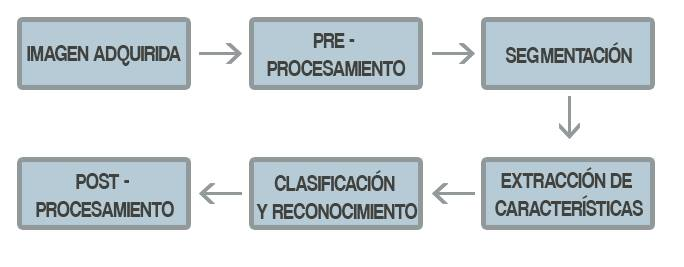
\includegraphics[scale=0.5]{img/OCR_pipeline_1.jpg} }
				\caption[Pipeline de procesamiento]{Esto es un ejemplo de como quedaría visualmente pero no es el pipeline de este trabajo.}
				\label{fig: Pipeline de mi sistema}
			\end{figure}

		\paragraph{Conjunto de entrenamiento} ~\\
		
			La primera etapa de este pipeline de procesamiento es la obtención de un conjunto de entrenamiento que se va a utilizar para entrenar al clasificador por lo que es imporante tener una buena cantidad de imágenes ya que esto impacta en la performance de reconocimiento. Este trabajo hace uso del dataset \textit{Chars74k} \cite{dCBV09} del cual se generan todos los conjuntos de entrenamiento que se utilizan en los experimentos. Se destacan dos grupos de imágenes al momento de entrentar, el de  caracteres segmentados de escenas naturales y el de caracteres sintéticos. El primero viene incluido en el dataset nombrado, en cambio, el segundo, tiene que ser generado como se procederá a explicar a continuación.
			

		\paragraph{Generación de datos sintéticos} ~\\

			La datos sintéticos que se generan y utilizan en este trabajo son extraidos del dataset \textit{Chars74K} el cual está compuesto, entre otras cosas, por 62992 imágenes de caracteres sintéticos extraidos de fuentes de computadora. Cada una de las clases involucradas en la clasificación tienen un poco más de 1000 de estas imágenes (son 62 clases en total). El objetivo detrás de la generación de estos datos sintéticos es agregar vistas de los caracteres que no están reflejadas en el dataset original pero que son plausibles de ser observadas en la realidad.
			
			Inicialmente, se tiene como base un conjunto el cual contiene imágenes de caracteres de diversas fuentes. Lo que se busca, es aplicar a cada imagen un conjunto de transformaciones afines aleatorias con el objetivo final de obtener una imagen nueva con la apariencia  lo más cercana a una real. Una transformación afin consiste en una transformación lineal seguida de una traslación. Formalmente, cada transformación afín es de la forma $x\mapsto Mx + b$, donde $M$ es una transformación lineal y $b$ es un vector. Se usan las multiplicaciones entre matrices para representar las transformaciones lineales y la suma de vectores para representar las traslaciones. Mediante matrices ampliadas, sin embargo, es posible representar ambos tipos de transformaciones.	La matriz $M$ presentada anteriormente es una matriz $2\times 2$ y permite realizar transformaciones en imágenes de 2 dimensiones. En este trabajo, para generar los datos sintéticos se hacen uso de las siguientes transformaciones:
			
			\paragraph{Rotación}
			
				La rotación es una transformación afín que consta en rotar el ángulo de la imágen en el sentido anti-horario. El parámetro usado para el mismo son los radianes y las diferentes variaciones se pueden apreciar en la figura \ref{fig: Transformacion Afin - Rotacion}. Teniendo en cuenta la definición formal de una transformación afín anterior, la rotación formalmente se puede representar de la siguiente manera:

			\begin{equation*}
					M =  
					\begin{bmatrix}
						cos(\theta) & -sin(\theta) \\
						sin(\theta) & cos(\theta)  \\
					\end{bmatrix}
					b =
					\begin{bmatrix}
						0 \\
						0 \\
					\end{bmatrix}	
			\end{equation*}

	donde se puede observar el parámetros $\theta$ que representa el grado de inclinación y el vector $b$ es nulo por lo cual no hay traslación alguna.

		\begin{figure}[htbp]
			\centering
			\subfloat[\label{fig: sintetica original}]{
				\fbox{ 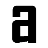
\includegraphics[scale=1]{img/transformaciones/original.png} }
			}
			\subfloat[\label{fig: Imagen rad 0.5}]{
				\fbox{ 
\includegraphics[scale=1]{img/transformaciones/rotation0,5.png} }
			}
			\subfloat[\label{fig: Imagen rad 1}]{
				\fbox{ 
\includegraphics[scale=1]{img/transformaciones/rotation1.png} }
			}
			\subfloat[\label{fig: Imagen rad 1.5}]{
				\fbox{ 
\includegraphics[scale=1]{img/transformaciones/rotation1,5.png} }
			}
			\caption[Rotación de un caracter]{Rotación de un caracter. (a) Imagen original. (b) Imagen rotada 0.5 radianes. (c) Imagen rotada 1 radian. (d) Imagen rotada 1.5 radianes}
			\label{fig: Transformacion Afin - Rotacion}
		\end{figure}	
			
		\paragraph{Escala}
			
			La escala es una transformación que busca modificar el tamaño del objeto al cual se la aplica haciendola más chica o más grande lo que era originalmente. Formalmente, se puede representar por la siguiente configuración de la matriz $M$:
			\begin{equation}
				M = 
				\begin{bmatrix}
					a & 0 \\
					0 & d \\
				\end{bmatrix}
			\end{equation}
		donde $a$ y $d$ representan los cambios en los ejes $x$ e $y$ de la imagen respectivamente. Se puede apreciar la aplicación de esta transformación en la figura \ref{fig: Transformacion Afin - Escala}.
		\begin{figure}[htbp]
			\centering
			\subfloat[\label{fig: escala original}]{
				\fbox{ 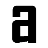
\includegraphics[scale=1]{img/transformaciones/original.png} }
			}
			\subfloat[\label{fig: Imagen escala 0.8}]{
				\fbox{ 
\includegraphics[scale=1]{img/transformaciones/scale0,8.png} }
			}
			\subfloat[\label{fig: Imagen escala 1.2}]{
				\fbox{ 
\includegraphics[scale=1]{img/transformaciones/scale1,2.png} }
			}
			\caption[Cambio de escala de un caracter]{Cambio de escala de un caracter. (a) Imagen original. (b) Imagen ampliada $1.2$ veces su tamaño  (c) Imagen reducida a $0.8$ veces su tamaño .}
			\label{fig: Transformacion Afin - Escala}
		\end{figure}	
			
		\paragraph{Transvección}
		
			La transvección es una transformación donde la imagen se rota en un solo eje. Es una función que toma un punto con coordenadas $(x,y)$ al punto $(x +ny, y)$ donde $n$ es un parámetro fijo, denominado el factor de inclinación. El efecto es el desplazamiento de todos los puntos horizontalmente en una cantidad proporcional a su coordenada $y$. Todo punto encima del eje $x$ es desplazado a la derecha si $n > 0$, y a la izquiera si $n < 0$. Nuestra matriz $M$ va a ser de la forma:
			\begin{equation}
				M = 
				\begin{bmatrix}
					1 & n \\
					0 & 1 \\
				\end{bmatrix}.
			\end{equation}
		Se puede observar en la figura \ref{fig: Transformacion Afin - Transveccion} los diferentes efectos de aplicar diferentes valores de $n$ en la aplicación de la transvección en una imagen.
		\begin{figure}[htbp]
			\centering
			\subfloat[\label{fig: Imagen transveccion 0.5}]{
				\fbox{ 
\includegraphics[scale=1]{img/transformaciones/shear0,5.png} }
			}
			\subfloat[\label{fig: Imagen transveccion 0.2}]{
				\fbox{ 
\includegraphics[scale=1]{img/transformaciones/shear0,20.png} }
			}
			\subfloat[\label{fig: Imagen original}]{
				\fbox{ 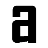
\includegraphics[scale=1]{img/transformaciones/original.png} }
			}
			\subfloat[\label{fig: Imagen transveccion -0.2}]{
				\fbox{ 
\includegraphics[scale=1]{img/transformaciones/shear-0,20.png} }
			}
			\subfloat[\label{fig: Imagen transveccion -0.5}]{
				\fbox{ 
\includegraphics[scale=1]{img/transformaciones/shear-0,5.png} }
			}
			\caption[Transvección de un caracter]{Transvección de un carácter.}
			\label{fig: Transformacion Afin - Transveccion}
		\end{figure}	
		
		\paragraph{Traslación}		
			
			La traslación es el último tipo de transformación afín que usamos en este trabajo y a diferencia del resto de las transformaciones, esta no hace uso de $M$, sino de $b$ que es el vector de desplazamiento. Formalmente:
			\begin{equation*}
				M =  
					\begin{bmatrix}
						1 & 0 \\
						0 & 1  \\
					\end{bmatrix}
					b =
					\begin{bmatrix}
						b_1 \\
						b_2 \\
					\end{bmatrix}	
			\end{equation*}
		donde $b_1$ y $b_2$ representan el movimiento en el eje $x$ e $y$ respectivamente. Particularmente no usamos esta transformación para mover los caracteres, sino más bien para mantener la imagen del carácter centrada durante las diferentes transformaciones que le aplicamos a la imagen.
		
		\paragraph{Otras transformaciones:} ~\\
		\paragraph{Suavizado Gaussiano}
		
			Es una técnica que consta de la difuminación de una imagen a partir de la convolución con una función gaussiana. Se usa principalmente para reducir el ruido en una imagen. Dados das las coordenadas de un punto $(x, y)$ en una imagen, la función de suavizado es la siguiente
			\begin{align*}
				G(x,y) = \frac{1}{2\pi\sigma^2}\epsilon^{-\frac{x^2+y^2}{2\sigma^2}}
			\end{align*}
			donde $\sigma$ es la desviación estandard de la distribución gaussiana. En la figura \ref{fig: Suavizado Gaussiano}, se puede observar como distintos valores para $\sigma$ a medida que aumenta va distorcionando la imagen un poco más.
			
		\begin{figure}[htbp]
			\centering
			\subfloat[\label{fig: Imagen original sin blur	}]{
				\fbox{ 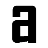
\includegraphics[scale=1]{img/transformaciones/original.png} }
			}
			\subfloat[\label{fig: Imagen con blur 1}]{
				\fbox{ 
\includegraphics[scale=1]{img/transformaciones/blur1.png} }
			}
			\subfloat[\label{fig: Imagen con blur 2}]{
				\fbox{ 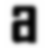
\includegraphics[scale=1]{img/transformaciones/blur2.png} }
			}
			\caption[Suavizado Gaussiano de un caracter]{Aplicación de blur o suavizado gaussiano a un caracter. (a) Imagen original. (b) Imagen suavizada con un valor de $\sigma = 1$  (c) Imagen aún más suavizada con un valor de $\sigma = 2$ .}
			\label{fig: Suavizado Gaussiano}
		\end{figure}				
			
			
		\paragraph{Ruido Gaussiano}			
			
			El ruido en una imagen es una variación en la información sobre el color o la iluminación en la misma. Puede ser producido por un sensor, la circuitería de una escaner o una cámara digital. Condiciones de poca iluminación o interferencia electromagnética durante la transmisión de las imágenes son factores para que aparezca este tipo de distorsiones. El ruido gaussiano en las imágenes es un tipo de ruido que se caracteríza por tener una distribución gaussiana. La figura \ref{fig: Ruido Gaussiano} presenta 2 ejemplos de imágenes de caracteres con ruido gaussiano. A medida que el parámetro $\sigma$  aumenta, el ruido en la imagen se hace más notorio.
			
		\begin{figure}[htbp]
			\centering
			\subfloat[\label{fig: Imagen original sin ruido	}]{
				\fbox{ 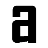
\includegraphics[scale=1]{img/transformaciones/original.png} }
			}
			\subfloat[\label{fig: Imagen con ruido 15}]{
				\fbox{ 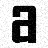
\includegraphics[scale=1]{img/transformaciones/noise15.png} }
			}
			\subfloat[\label{fig: Imagen con ruido 30}]{
				\fbox{ 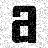
\includegraphics[scale=1]{img/transformaciones/noise30.png} }
			}
			\caption[Ruido Gaussiano en un caracter]{Aplicación de ruido gaussiano a un caracter. (a) Imagen original. (b) sigma=15  (c) sigma=30 .}
			\label{fig: Ruido Gaussiano}
		\end{figure}
			
			Un punto a destacar en este proceso, es que las fuentes de letras están en una escala de grises y se mantienen de esta forma. Esto es debido a que, durante el entrenamiento, solo es posible obtener las características de las imágenes sí y sólo sí estas están en escala de grises (requerimiento del algoritmo HOG). 
			
			
			%\paragraph{Anexar caracteres}
					
			%Otro tipo de modificación que vale la pena destacar, es la de anexar caracteres a los costados de la imagen a alterar. Esto es debido a que la mayoría de las imágenes de caracteres reales son extraidas de entornos donde la misma forma parte de una palabra. Es por eso que en la mayoría de los conjuntos generados, cada caracter está acompañado de pedazos de otros caracteres.
			
		%\begin{figure}[htbp]
		%	\centering
		%	\subfloat[\label{fig: Imagen anexo 1	}]{
		%		\fbox{ 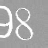
\includegraphics[scale=1]{img/transformaciones/anexo1.png} }
		%	}
		%	\subfloat[\label{fig: Imagen anexo 2}]{
		%		\fbox{ 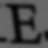
\includegraphics[scale=1]{img/transformaciones/anexo2.png} }
		%	}
		%	\subfloat[\label{fig: Imagen anexo 3}]{
		%		\fbox{ 
\includegraphics[scale=1]{img/transformaciones/anexo3.png} }
		%	}
		%	\caption[Caracteres pegados]{Imágenes de caracteres con caracteres pegados a izquierda y derecha.}
		%	\label{fig: Imagen anexos}
		%\end{figure}

		%	La creación de estos datos sintéticos son para el conjunto de entrenamiento del clasificador. El conjunto de test esta conformado por 15 imágenes reales por clase obtenidas del dataset \textit{Chars74K-15}, a las cuales no se les modifico en absoluto.

		\paragraph{Extracción de características y binarización} ~\\
		
			La siguiente etapa en el pipeline es la extracción del vector de características (ver sección ``Vectores de características'' \ref{subsection:feature}) de cada imagen del conjunto de entrenamiento y la binarización posterior de dicho descriptor (ver sección ``Binarización'' \ref{subsection:hog}).
			
			Una de las condiciones para poder extraer el vector de características de una imagen con HOG, es que esta esté en escala de grises o en blanco y negro. Luego, dado un conjunto de entrenamiento con $J$ imágenes, se construye una matriz $J \times K$ donde $K$ es la dimensión del descriptor HOG para cada imagen. Cabe aclarar que todas las imágenes tienen que tener las mismas dimensiones (48x48 píxeles) de lo contrario no se podría construir la matriz. Esto se debe a que HOG devuelve en sí un vector $v \in \mathbb{R}^{K}$ (donde $K$ depende de los parámetros que se le pasen al algoritmo y a la dimensión de la imagen). Posteriormente se procede como se detalla en \ref{subsection:hog} donde se obtiene el umbral que después se utiliza para binarizar todos los descriptores tanto del conjunto de entrenamiento como del conjunto de evaluación.
			
		

		\paragraph{Entrenamiento del clasificador}  ~\\

			En esta etapa, al igual que los autores del trabajo original, se utiliza como clasificador a Random Ferns. Para poder entrenar al clasificador, los vectores modificados de la etapa anterior se almacenan en un diccionario. Este último, esta estructurado como un conjunto de diccionarios anidados y representa la ``base de datos'' del sistema. Los detalles del porqué se eligió esta forma de almacenar la información se puede encontrar en el apéndice A. \RC{Crear apendice A donde se van a discutir cosas como lenguaje usado, base de datos, librerias entre otros}

			Dado que los vectores binarizados pertenecen al conjunto $\{ 0,1 \}^{N}$ si los quisiéramos almacenar en una sola tabla (habría una tabla por clase), cada una debería tener $2^{N}$ entradas lo cual si $N$ es muy grande sería imposible por la cantidad de memoria necesitada para mantener estas tablas en memoria. Luego, basándonos en lo explicado sobre Random Fern en \cite{subsection:ferns}, la solución pasa por dividir cada vector en $M$ grupos de dimensión $S = \frac{N}{M}$. Con esto, un vector completo esta almacenado en $M$ tablas diferentes (tablas correspondiente a la clase del vector). En total estaríamos trabajando con $M \times 62$ tablas (pues hay 62 clases diferentes).

			Dado un vector $v=(v_1, \dots, v_s)$ donde $v_i \in \{ 0,1 \}^{M}$, $z$ sea la clase de $v$ y sean $t_i i=1, \dots, s$ las tablas de $z$. Cada grupo $v_i i=1, \dots, s$ va a tener una entrada en su tabla correspondiente $z_i$ equivalente a su representación decimal. Inicialmente cada tabla está inicializada dado un parámetro $\alpha \neq 0$ que se explicará en detalle en el próximo capítulo.

		\paragraph{Evaluación del clasificador} ~\\

			Para la evaluación del clasificador, se toma como conjunto de test el descripto en la sección de descripción del dataset. A cada imágen del conjunto de test, se le extrae el descriptor HOG, se lo binariza y con el vector resultante se calcula la probabilidad de que dicho vector perteneza a cada una de las clases involucradas. El calculo para cada clase es el mismo y consiste en dividir el vector de prueba en $M$ grupos y por cada grupo obtener el valor en la tabla correspondiente. Por cada clase entonces tendríamos $M$ valores. Finalmente se realiza la suma de los logaritmos de cada valor y el resultado es la probabilidad de que ese vector pertenzca a la clase evaluada. Como es claro, al final se le asigna a la imagen evaluada la clase que haya obtenido la mayor probabilidad.

